\section{Background and Related Work}
\label{sec:background}

In this section, we describe relevant background and related work. We first
provide background on Merkle hash trees and \acl{ct}, both of which we refer to
in the remainder of the paper. We then discuss related work from both the
academic literature and projects from the industry and open-source communities
and their shortcomings. We then examine previous work that has addressed the
problem of specifying or inferring a domain's certificate policy. We conclude by
examining work that has addressed the problem of signaling HTTPS deployment in
domains.

\subsection{Merkle Hash Trees}
\label{sec:background:mht}

\begin{figure}
  \centering
  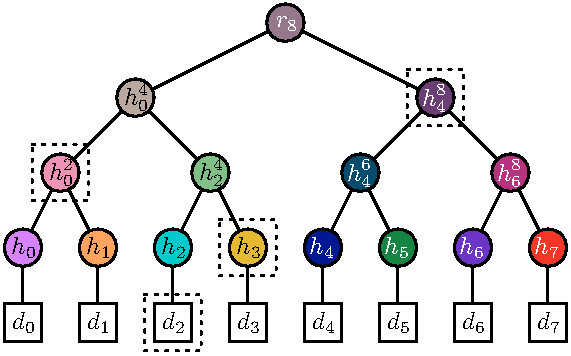
\includegraphics[width=\linewidth]{fig/mht-audit}
  \caption{Sample Merkle hash tree with eight leaf nodes. Dashed boxes indicate
  the nodes sent to prove the presence of the leaf $d_2$ in the tree.}
  \label{fig:mht-audit}
\end{figure}

A \emph{Merkle hash tree} is a binary tree in which each leaf node's value
represents data and each non-leaf node's value is the hash of its children's
values~\cite{merkle1988digital}. As shown in \autoref{fig:mht-audit}, the
structure of a Merkle hash tree allows one to efficiently prove that a data item
is present in the tree. Specifically, given the value of the root node of the
tree, one can verify the presence of any leaf node in the tree by computing a
number of hashes that is logarithmic in the number of data items in the tree.

A Merkle hash tree can store any number of nodes, i.e., the tree does not need
to be balanced. While several ways of computing the hashes in a non-balanced
tree exist, in this paper we use the method used in \ac{ct}~\cite{rfc6962}.
Specifically, given $n$ items in the Merkle hash tree, let \hashfunc be a hash
function, $d_i$ the $i$th data item (indexed from 0), and $a$ and $b$ integers
such that $0 < a < b \le n$. Then the hash of a non-leaf node representing the
$a$th to the $(b-1)$th data items is defined as
\begin{equation}
  \nodehash_a^b =
  \begin{cases}
    \hashfunc(0 \| d_a) & \mathrm{if\ } b = a + 1 \\
    \hashfunc(1 \| \nodehash_a^k \| \nodehash_k^b) & \mathrm{otherwise}
  \end{cases}
\end{equation}
where $\|$ denotes concatenation and $k = a + 2^{\lceil \log_2(b-a) \rceil - 1}$
(the largest power of 2 strictly less than $b - a$). For convenience, if $b = a
+ 1$ we write the hash as $\nodehash_a$ and call this a \emph{leaf hash}, and if
$a = 0$ and $b = n$ then we write the hash as $r_n$ and call this the \emph{root
hash}.

\begin{figure}
  \centering
  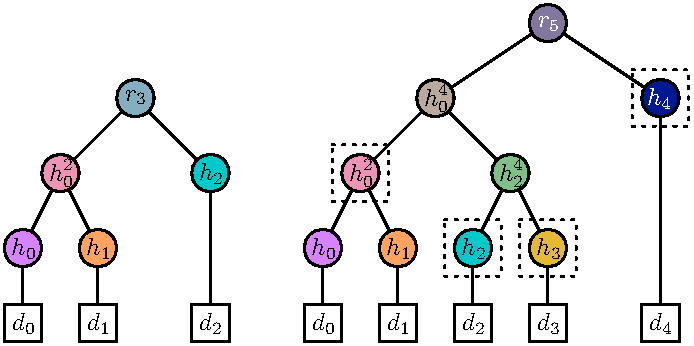
\includegraphics[width=\linewidth]{fig/mht-consistency}
  \caption{Sample Merkle hash trees with three and five data items,
  respectively. Dashed boxes indicate the nodes sent to prove consistency
between the root hashes $r_3$ and $r_5$.}
  \label{fig:mht-consistency}
\end{figure}

A Merkle hash tree can be used to implement an append-only, tamper-proof
log~\cite{crosby2009efficient}. As stated above, a Merkle hash tree can provide
an efficient \emph{proof of presence} for a given data item in the tree, thus
proving that an item was logged. To prove that the log is append-only, that is,
that no items have been changed or removed from the log, we can also use a
Merkle hash tree to provide an efficient \emph{proof of consistency} that is
logarithmic in the current size of the tree. As shown in
\autoref{fig:mht-consistency}, a proof of consistency allows one to compute the
root hash at two different times, thus showing that nodes have only been added
to the tree. A tamper-proof log would periodically sign and broadcast its root
hash, allowing clients to verify that it is not tampering with previously logged
data.

\subsection{Certificate Transparency}
\label{sec:background:ct}

\begin{figure}
  \centering
  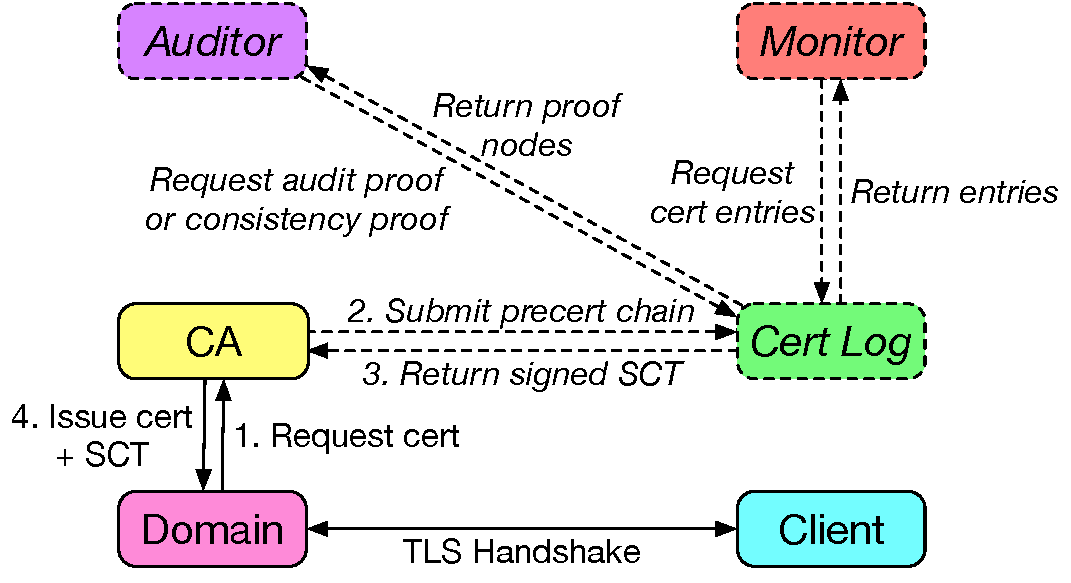
\includegraphics[width=\linewidth]{fig/ct}
  \caption{One possible configuration of the \ac{ct} architecture. Numbered
  steps denote the certificate issuance process. Dashed lines and boxes denote
entities or functions introduced by \ac{ct}, with their descriptions in
italics.}
  \label{fig:ct}
\end{figure}

\acf{ct} is a project by Google focused on enabling widespread detection of
certificate issuance~\cite{rfc6962}. As shown in \autoref{fig:ct}, \ac{ct}
introduces several new roles to the \ac{ca}-based ecosystem. \emph{Certificate
logs} are entities who record \ac{ca} behavior by maintaining a publicly
auditable, append-only, tamper-proof database of certificates. \emph{Monitors}
periodically retrieve these certificates to check for suspicious \ac{ca}
behavior, such as an obscure \ac{ca} issuing a certificate for Google.
\emph{Auditors} check for correct log behavior by periodically asking for
\emph{audit proofs}, which show that one or more certificates are in a log
database, or \emph{consistency proofs}, which show that the existing database
has not been tampered with, i.e., that no certificate has been changed, deleted,
or retroactively added to the log database.

A log leverages Merkle hash trees to implement its certificate database. As
explained above, the use of a Merkle hash tree allows a log to provide efficient
proofs of presence (i.e., audit proofs) and proofs of consistency (i.e.,
consistency proofs). While anyone may submit a certificate to a log, in current
practice \acp{ca} usually log certificates during the issuance process, as
depicted in \autoref{fig:ct}. Because attempting to update the Merkle hash tree
in real time may delay or block the certificate issuance process, logs define a
\emph{\ac{mmd}}, a time period after which a certificate is guaranteed to be
logged, and instead return a \emph{\ac{sct}}, which is effectively a promise to
add the certificate within the \ac{mmd}. The \ac{sct} is embedded into the
\ac{ca}-issued certificate as an X.509 extension and used to signal that a
domain uses \ac{ct} and that its certificate has been logged. Alternately, the
domain can send extra information such as \acp{sct} or audit proofs in the
\ac{tls} handshake using a \ac{tls} protocol extension.

%\draft{Monitoring and auditing details. Monitors periodically downloads all new
  %entries and verifies consistency proof. Does not need to keep cert entries
  %after finishing. Auditors periodically query for random audit proofs or
  %consistency proofs. Specifically, can pass a cert hash and a size of the tree
  %and get an audit proof in return, or pass two sizes of the tree and get a
  %consistency proof in return. To verify this information, log also provides a
  %function to get the latest signed tree head. In order to detect
  %\emph{equivocation} (i.e., showing different versions of the log to different
  %queries), auditors must gossip tree heads. The log's public key is known
  %through a trusted entity such as Google.}

%\draft{\ac{ct} does not check for revocation, though multiple extensions
%designed to handle revocation have been proposed (see \autoref{sec:related}).
%Perhaps the easiest way to do to this is to create a new Merkle hash tree every
%\ac{mmd} that contains as its leaves the list of \emph{currently valid}
%certificates.}

\subsection{Specifying and Inferring Domain Policy}
\label{sec:background:policy}

Previous work has proposed the use of domain-specified policies to protect
against \ac{mitm} attacks. In AKI~\cite{kim2013accountable} and its successor
ARPKI~\cite{basin2014arpki}, these policies are embedded within the certificates
themselves and specify attributes such as trusted \acp{ca} and public logs as
well as a ``cool-off period'' that forces potentially malicious certificates to
be visible in logs for some period of time before client can accept them. In
PoliCert~\cite{szalachowski2014policert}, the policies are stored separately in
logs. Other work, such as Blockstack~\cite{ali2016blockstack} or
IKP~\cite{matsumoto2017ikp}, has proposed placing policy information into a
blockchain. While IKP's policies operate similarly to those of PoliCert,
Blockstack simply provides the domain's keys directly. Of these proposals, only
ARPKI leverages the relationship between \acp{ca} and logs to ease the burden on
the domain during certificate issuance, but all proposals require the domain to
specify its policy in detail to prevent \ac{mitm} attacks resulting from
misbehaving \acp{ca}.

There has also been some work that takes a heuristic approach, using the past
behavior of \acp{ca} in order to determine how clients should trust them. For
example, CAge~\cite{kasten2013cage} propose a system that displays a browser
warning to users for certificates whose names are under a DNS top-level domain
that the issuing \ac{ca} has never signed for before. Perl, Fahl and Smith
propose to outright remove root certificates that have not been used to sign
(either directly or through \ac{ca} delegation) any observed certificates in the
past~\cite{perl2014you}. Both of these proposals use data from
Censys~\cite{durumeric2015search} or its predecessors, but do not use any
information from the domains themselves. Because of this, these approaches may
encounter situations where they mistake a legitimate, domain-initiated change
with an attempted \ac{mitm} attack and thus block a user from visiting a benign
site or expose a user to the \ac{mitm} attack. Indeed, a previous study of
changes in the Web \ac{pki}'s trust graph suggests that legitimate changes and
attacks share properties to the point that they cannot be easily
distinguished~\cite{amann2013no}.

\subsection{Signaling \ac{https} Deployment}
\label{sec:background:signaling}

Although \ac{hsts}~\cite{rfc6797} enforces the use of \ac{https} for a site
after a client has connected with that site over \ac{https} for the first time,
previous work has acknowledged the difficulty (in terms of both storage and
latency overhead) of identifying \ac{https}-deploying domains before the first
visit. The prevailing solution among browser vendors is \emph{\ac{hsts}
preloading}~\cite{keeler2012preloading}, in which browser vendors include a list
of the most popular sites that have deployed \ac{https}. These lists are
incomplete (covering only \steve{TODO: fill in} names in Chrome), and domains
must explicitly opt into adding themselves. As indicated by vendor-provided
guidelines,\footnote{\url{https://hstspreload.org/}} this process is prone to
mistakes by domain operators that lead to site inaccessibility.

As described in \steve{TODO: refer to previous section if mentioned elsewhere},
most approaches to disseminating certificate revocation information fail for
signaling because they rely on assumptions that do not hold in the signaling
problem. In particular, the use of \acp{crl}~\cite{rfc5280} does not scale to
the number of \ac{https}-deploying sites because we cannot assume that the
number of sites deploying \ac{https} will remain small compared to the overall
number of sites. More efficient versions of \acp{crl} also do not work: an
approach similar to Chrome's CRLsets~\cite{langley2012revocation} suffers from
the same incompleteness and opt-in hurdles mentioned above, and an approach
similar to CRLite~\cite{larisch2017crlite} relies on knowledge of all domain
names, which is infeasible in today's DNS due to many country code top-level
domains keeping their registries private. Approaches such as storing data in a
2-3 tree~\cite{naor1998certificate} or aoptimized Merkle hash
tree~\cite{laurie2012revocation}, while able to provide efficient proofs of
\ac{https} deployment, require online checks by clients, greatly increasing the
latency of connection establishment.

DANE~\cite{rfc6698}, which uses DNS to send a public key, certificate, or
\ac{ca} that the client should expect, can provide both signaling and policy
management with little added latency and without requiring browsers to store any
kind of signaling information. However, DANE relies on DNSSEC~\cite{rfc4033},
and both have a low deployment rate in today's Internet. Since DANE's
standardization in 2011 and DNSSEC's in 2005, only 5,885 DANE records for
\ac{https} and 1.67M verified DNSSEC zones out of more than 329M names
overall~\cite{dnib-14-1}
exist.\footnote{\url{http://secspider.verisignlabs.com/stats.html}, retrieved 1
August 2017} Changing these numbers would require significant deployment efforts
on the parts of domains, including registering domain names through the subset
of DNS registrars that offer DNSSEC, usually as a paid service.
